\subsection{Constraint Mapping Performance}
\label{sec:constraintextraction}

Our second experiment evaluates how model and mapper choices affect mapping quality. To isolate mapping from classification errors, we compute constraint extraction and aggregate violation F$_1$ on the ground-truth constraint sentences only, comparing the \emph{Single-Prompt} and \emph{Multi-Step} mappers with six LLMs (Figure~\ref{fig:mapper-results}, Table~\ref{tab:mapping-metrics}). On Hospital, Restaurant, SISU, and Tax, \emph{Multi-Step} improves both metrics (mean over models: 0.81 vs.\ 0.75 and 0.83 vs.\ 0.55), with the largest gains on Restaurant and SISU, whose rules combine several conditions or relate two tuples. The best Multi-Step configurations exceed the best one of the preliminary study (GPT-5, 0.78 and 0.95): Claude Sonnet 5.5 reaches 0.85 and 0.97, GPT-6 Luna 0.82 and 0.98, and Qwen3.8-2.4T-A95B 0.80 and 1.00. Decomposition also keeps the mapper usable with unstable backbones: MiniMax-M3 returned empty outputs for 107 of 156 Single-Prompt sentences but completed the Multi-Step pipeline without failures; among the final backbones, only DeepSeek-V4-Flash has output failures (3 Single-Prompt sentences).

\begin{figure}[!ht]
    \centering
    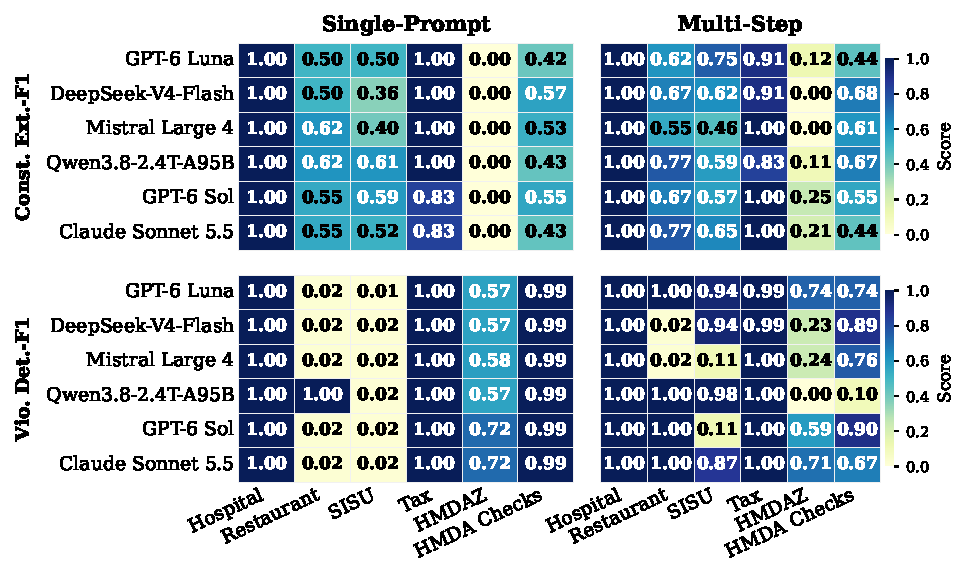
\includegraphics[width=\columnwidth]{figures/results/v3_fig7_mapping.pdf}
    \caption{Sentence-level mapping results across models and mappers: constraint extraction F$_1$ and aggregate violation F$_1$ on ground-truth sentences.}
    \label{fig:mapper-results}
\end{figure}

\smallskip\noindent\textbf{Where Single-Prompt loses violations.}
On Restaurant, one rule (at least one inspection per year) flags 99\% of the gold-violating tuples. Every Single-Prompt configuration except Qwen3.8-2.4T-A95B returns \texttt{null} for it, so aggregate recall falls to 0.01; without this rule, all reach 1.00. On SISU, Single-Prompt identifies the student by the exam registration number instead of the national ID in the two-tuple rules, flagging about 51k tuples instead of 533. Multi-Step, which links columns and selects predicates before writing the DC, avoids both errors with most backbones, but not all: DeepSeek-V4-Flash and Mistral Large 4 also miss the Restaurant rule, and GPT-6 Sol and Mistral Large 4 make the identification error in one SISU rule (8.9k tuples; aggregate 0.11).

\begin{table}[!ht]
  \centering
  \small
  \setlength{\tabcolsep}{3.5pt}
  \resizebox{\columnwidth}{!}{\begin{tabular}{llrrrrrr}
\toprule
\textbf{Mapper} & \textbf{Model} & CM & CM$_{\equiv}$ & AV & Rule-F$_1$ & Exec. & Fail. \\
\midrule
\multirow{6}{*}{Single-Prompt} & GPT-6 Luna & 0.57 & 0.69 & 0.60 & 0.78 & 0.75 & 0 \\
 & DeepSeek-V4-Flash & 0.57 & 0.66 & 0.60 & 0.74 & 0.70 & 3 \\
 & Mistral Large 4 & 0.59 & 0.66 & 0.60 & 0.73 & 0.71 & 0 \\
 & Qwen3.8-2.4T-A95B & 0.61 & 0.70 & 0.76 & \textbf{0.86} & \textbf{0.83} & 0 \\
 & GPT-6 Sol & 0.59 & 0.67 & 0.62 & 0.76 & 0.72 & 0 \\
 & Claude Sonnet 5.5 & 0.55 & 0.64 & 0.62 & 0.76 & 0.70 & 0 \\
\midrule
\multirow{6}{*}{Multi-Step} & GPT-6 Luna & 0.64 & 0.69 & \textbf{0.90} & 0.77 & 0.76 & 0 \\
 & DeepSeek-V4-Flash & 0.65 & 0.69 & 0.68 & 0.68 & 0.69 & 0 \\
 & Mistral Large 4 & 0.60 & 0.64 & 0.52 & 0.74 & 0.73 & 0 \\
 & Qwen3.8-2.4T-A95B & 0.66 & 0.68 & 0.68 & 0.81 & 0.77 & 0 \\
 & GPT-6 Sol & 0.67 & 0.71 & 0.77 & 0.79 & 0.77 & 0 \\
 & Claude Sonnet 5.5 & \textbf{0.68} & \textbf{0.74} & 0.88 & 0.84 & 0.82 & 0 \\
\bottomrule
\end{tabular}
}
  \caption{Mean mapping quality over the six datasets (ground-truth sentences). CE: exact extraction F$_1$; CE$_{\equiv}$: equivalence-aware extraction F$_1$; AV: aggregate violation F$_1$; Rule-F$_1$: mean per-rule violation F$_1$; Exec.: execution equivalence; Fail.: sentences with no valid output.}
  \label{tab:mapping-metrics}
\end{table}

\smallskip\noindent\textbf{HMDA datasets.}
Exact extraction stays low (at most 0.25 on HMDAZ and 0.68 on HMDA Checks). Many predicted DCs are logically equivalent to the gold ones but written differently (\texttt{IN} instead of a disjunction, a label instead of its code column); others omit the coverage conditions of a trigger. Equivalence-aware extraction recovers much of the first group: on the HMDA datasets it raises mean extraction F$_1$ from 0.34 to 0.46 for Multi-Step and from 0.24 to 0.51 for Single-Prompt, while it barely changes elsewhere. On HMDA Checks, aggregate violation is not informative: two date-range edits flag 99\% of the gold-violating tuples, which cover 98.6\% of the rows, so a DC flagging every tuple already scores 0.99. Single-Prompt reaches 0.99 with every backbone, mostly through such DCs. Multi-Step scores 0.67--0.90 with five backbones, but only GPT-6 Sol maps a date edit correctly; the others write incorrect DCs for other edits that flag 480k--550k rows and pass the 90\% violation-share check. Without the two date edits, the Multi-Step aggregate falls to 0.12--0.19 for four backbones and stays at 0.98--1.00 for GPT-6 Sol and Qwen3.8-2.4T-A95B, while Single-Prompt ranges from 0.18 to 1.00. Per-rule metrics are far less sensitive: mean per-rule F$_1$ is 0.78 (Multi-Step) and 0.86 (Single-Prompt) with all edits, and 0.84 and 0.85 without the date edits.

\smallskip\noindent\textbf{Default mapper and sensitivity to the backbone.}
With Multi-Step, Claude Sonnet 5.5 has the best mean extraction (0.68) and GPT-6 Luna the best mean aggregate violation (0.90). The mean of the two selects \emph{Claude Sonnet 5.5} (0.776, against 0.771 for GPT-6 Luna and 0.720 for GPT-6 Sol), a tie with GPT-6 Luna given single runs. Backbones differ more in violation detection than in extraction: mean exact extraction ranges only from 0.60 to 0.68, aggregate violation from 0.52 to 0.90, and per-rule metrics lie in between (0.68--0.84). The divergences concentrate on implicit decisions rather than syntax: which attribute identifies an entity (SISU), whether a definition implies a checkable trigger (HMDAZ), and how integer-encoded dates are compared (HMDA Checks). Single runs also vary: two runs of Mistral Large 4 on Restaurant, differing only in a check unrelated to the dominant rule, scored 1.00 and 0.02 in aggregate because that rule was mapped in one run only. We cannot relate these differences to model size or training data, which most backbones do not disclose.
